\documentclass[journal]{IEEEtran}

\ifCLASSINFOpdf

\else

\fi

\hyphenation{op-tical net-works semi-conduc-tor}
\usepackage{graphicx}
\usepackage{bm}
\usepackage{siunitx}
\usepackage{tikz}
\usetikzlibrary{intersections, calc}
\graphicspath{ {img/} }
\pagenumbering{gobble}
\newcommand*{\subb}[1]{_{\mathrm{#1}}}
\tikzset{
	partial ellipse/.style args={#1:#2:#3}{
		insert path={+ (#1:#3) arc (#1:#2:#3)}
	}
}

\begin{document}
	% paper title
	% can use linebreaks \\ within to get better formatting as desired
	% Do not put math or special symbols in the title.
	\title{Motion Control of Unmanned Aerial Vehicle}
	\author{Vilhelm~Dinevik and Paula~Carb\'o}
	% author names and IEEE memberships
	% note positions of commas and nonbreaking spaces ( ~ ) LaTeX will not break
	% a structure at a ~ so this keeps an author's name from being broken across
	% two lines.
	% use \thanks{} to gain access to the first footnote area
	% a separate \thanks must be used for each paragraph as LaTeX2e's \thanks
	% was not built to handle multiple paragraphs
	%
	
	
	
	% note the % following the last \IEEEmembership and also \thanks -
	% these prevent an unwanted space from occurring between the last author name
	% and the end of the author line. i.e., if you had this:
	%
	% \author{....lastname \thanks{...} \thanks{...} }
	%                     ^------------^------------^----Do not want these spaces!
	%
	% a space would be appended to the last name and could cause every name on that
	% line to be shifted left slightly. This is one of those "LaTeX things". For
	% instance, "\textbf{A} \textbf{B}" will typeset as "A B" not "AB". To get
	% "AB" then you have to do: "\textbf{A}\textbf{B}"
	% \thanks is no different in this regard, so shield the last } of each \thanks
	% that ends a line with a % and do not let a space in before the next \thanks.
	% Spaces after \IEEEmembership other than the last one are OK (and needed) as
	% you are supposed to have spaces between the names. For what it is worth,
	% this is a minor point as most people would not even notice if the said evil
	% space somehow managed to creep in.
	
	
	% The paper headers
	\markboth{A3. Smart Autonomous Systems in Robotics}%
	{Shell \MakeLowercase{\textit{et al.}}: Bare Demo of IEEEtran.cls for Journals}
	% The only time the second header will appear is for the odd numbered pages
	% after the title page when using the twoside option.
	%
	% *** Note that you probably will NOT want to include the author's ***
	% *** name in the headers of peer review papers.                   ***
	% You can use \ifCLASSOPTIONpeerreview for conditional compilation here if
	% you desire.
	
	% make the title area
	\maketitle
	
	% As a general rule, do not put math, special symbols or citations
	% in the abstract or keywords.
	\begin{abstract}
		The abstract goes here.
	\end{abstract}
	
	% Note that keywords are not normally used for peerreview papers.
	\begin{IEEEkeywords}
		IEEEtran, journal, \LaTeX, paper, template.
	\end{IEEEkeywords}
	
	
	% For peer review papers, you can put extra information on the cover
	% page as needed:
	% \ifCLASSOPTIONpeerreview
	% \begin{center} \bfseries EDICS Category: 3-BBND \end{center}
	% \fi
	%
	% For peerreview papers, this IEEEtran command inserts a page break and
	% creates the second title. It will be ignored for other modes.
	%\IEEEpeerreviewmaketitle
	
	\section{Introduction}
	% The very first letter is a 2 line initial drop letter followed
	% by the rest of the first word in caps.
	%
	% form to use if the first word consists of a single letter:
	% \IEEEPARstart{A}{demo} file is ....
	%
	% form to use if you need the single drop letter followed by
	% normal text (unknown if ever used by IEEE):
	% \IEEEPARstart{A}{}demo file is ....
	%
	% Some journals put the first two words in caps:
	% \IEEEPARstart{T}{his demo} file is ....
	%
	% Here we have the typical use of a "T" for an initial drop letter
	% and "HIS" in caps to complete the first word.
	\IEEEPARstart{U}{nmanned} aerial vehicles, also known as UAVs, are becoming nowadays more and more popular because they are small, cheap to produce, have low operating and maintenance cost, have great maneuverability, can perform steady flight operations and are able to enter high-risk areas without having to compromise human safety. Most applications that involve UAVs have been used in open areas without any obstacles and with a human in control of the UAV. But in recent years people have come up with more modern applications of UAVs that will need UAVs to fly autonomously in densely populated areas, with a lot of other autonomous UAVs around, e.g. Amazon Prime Air delivery system, AltiGator drones services for inspection and data adquisition, or multi-UAVs used to deploy an aerial communications network. This places high demands on UAVs’ obstacle avoidance capabilities for both moving and static obstacles.
	
	There are many different manufacturers and a vast amount of different UAV models, all with different motors, weights, sensors and lift-to-weight ratio. To make a standard autonomous flight applicable to all these kinds of UAVs, a simple and easy-to-implement multi-UAV mathematical model, that will still be able to avoid obstacles with as few sensors as possible, is needed.
	
	This project aims to study and develop a mathematical model of a quadrotor UAV and the available sensors in it.  From the trajectory and pose tracking a state feedback controller will be designed. In order to facilitate the multi-UAV navigation, potential fields or an A* algorithm will be used to make several quads fly to their goals while maintaining collision avoidance with respect to other quads and obstacles. To check the validity of the models, a simulated test environment in MatLab filled with a random reasonable amount of static obstacles and autonomous UAVs will be used.
	% !TeX AoP in the introduction: We can consider improving this last paragraph, and expanding it so everything we do through the report is explained
	\hfill 
	
	
	%\subsection{The Issue}
	%How make super small propeller things not smash into each other or other things.
	%
	%% needed in second column of first page if using \IEEEpubid
	%%\IEEEpubidadjcol
	%
	%\subsubsection{Subsubsection of the Issue}
	%How do we do dis?.
	
	
	% An example of a floating figure using the graphicx package.
	% Note that \label must occur AFTER (or within) \caption.
	% For figures, \caption should occur after the \includegraphics.
	% Note that IEEEtran v1.7 and later has special internal code that
	% is designed to preserve the operation of \label within \caption
	% even when the captionsoff option is in effect. However, because
	% of issues like this, it may be the safest practice to put all your
	% \label just after \caption rather than within \caption{}.
	%
	% Reminder: the "draftcls" or "draftclsnofoot", not "draft", class
	% option should be used if it is desired that the figures are to be
	% displayed while in draft mode.
	%
	%\begin{figure}[!t]
	%\centering
	%\includegraphics[width=2.5in]{myfigure}
	% where an .eps filename suffix will be assumed under latex,
	% and a .pdf suffix will be assumed for pdflatex; or what has been declared
	% via \DeclareGraphicsExtensions.
	%\caption{Simulation Results.}
	%\label{fig_sim}
	%\end{figure}
	
	% Note that IEEE typically puts floats only at the top, even when this
	% results in a large percentage of a column being occupied by floats.
	
	
	% An example of a double column floating figure using two subfigures.
	% (The subfig.sty package must be loaded for this to work.)
	% The subfigure \label commands are set within each subfloat command,
	% and the \label for the overall figure must come after \caption.
	% \hfil is used as a separator to get equal spacing.
	% Watch out that the combined width of all the subfigures on a
	% line do not exceed the text width or a line break will occur.
	%
	%\begin{figure*}[!t]
	%\centering
	%\subfloat[Case I]{\includegraphics[width=2.5in]{box}%
	%\label{fig_first_case}}
	%\hfil
	%\subfloat[Case II]{\includegraphics[width=2.5in]{box}%
	%\label{fig_second_case}}
	%\caption{Simulation results.}
	%\label{fig_sim}
	%\end{figure*}
	%
	% Note that often IEEE papers with subfigures do not employ subfigure
	% captions (using the optional argument to \subfloat[]), but instead will
	% reference/describe all of them (a), (b), etc., within the main caption.
	
	
	% An example of a floating table. Note that, for IEEE style tables, the
	% \caption command should come BEFORE the table. Table text will default to
	% \footnotesize as IEEE normally uses this smaller font for tables.
	% The \label must come after \caption as always.
	%
	%\begin{table}[!t]
	%% increase table row spacing, adjust to taste
	%\renewcommand{\arraystretch}{1.3}
	% if using array.sty, it might be a good idea to tweak the value of
	% \extrarowheight as needed to properly center the text within the cells
	%\caption{An Example of a Table}
	%\label{table_example}
	%\centering
	%% Some packages, such as MDW tools, offer better commands for making tables
	%% than the plain LaTeX2e tabular which is used here.
	%\begin{tabular}{|c||c|}
	%\hline
	%One & Two\\
	%\hline
	%Three & Four\\
	%\hline
	%\end{tabular}
	%\end{table}
	
	
	% Note that IEEE does not put floats in the very first column - or typically
	% anywhere on the first page for that matter. Also, in-text middle ("here")
	% positioning is not used. Most IEEE journals use top floats exclusively.
	% Note that, LaTeX2e, unlike IEEE journals, places footnotes above bottom
	% floats. This can be corrected via the \fnbelowfloat command of the
	% stfloats package.
	
	\section{Quadcopter modelling}
	\subsection{Overview}
	\begin{figure}
		\centering
		% !TeX root=../Report.tex 
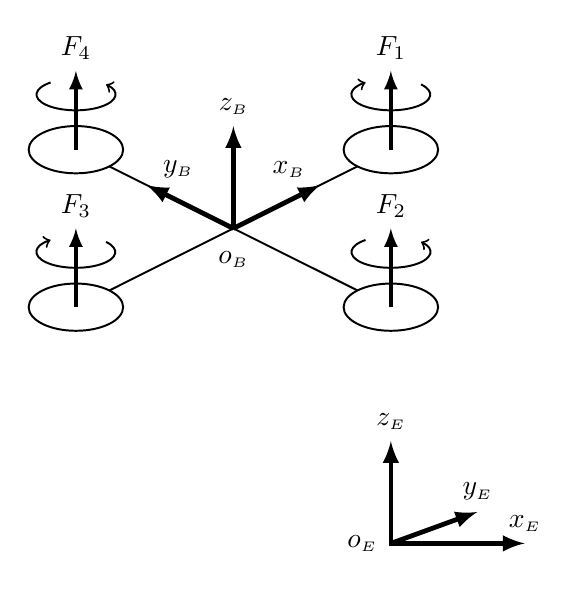
\begin{tikzpicture}
	\draw[line width=0.25mm, name path=eldownleft] (0,0) ellipse (0.6 and 0.3);
	\draw[line width=0.25mm, name path=eldownright] (4,0) ellipse(0.6 and 0.3);
	\draw[line width=0.25mm, name path=elupright] (4,2) ellipse (0.6 and 0.3);
	\draw[line width=0.25mm, name path=elupleft] (0,2) ellipse (0.6 and 0.3);
	
	\path [name path= downleft] (0,0) -- (2,1);
	\path [name path= upleft] (0,2) -- (2,1);
	\path [name path= downright] (4,0) -- (2,1);
	\path [name path= upright] (4,2) -- (2,1);
	
	\draw [name intersections={of=eldownleft and downleft}][line width=0.25mm] (intersection-1) --(2,1);
	\draw [name intersections={of=eldownright and downright}][line width=0.25mm] (intersection-1) -- (2,1);
	\draw [name intersections={of=elupright and upright}][line width=0.25mm] (intersection-1) -- (2,1);
	\draw [name intersections={of=elupleft and upleft}][line width=0.25mm] (intersection-1) -- (2,1);
	
	\draw[line width=0.45mm,-latex] (0,0) -- (0,1) node [above] {$F_3$};
	\draw[line width=0.45mm,-latex] (4,0) -- (4,1) node [above] {$F_2$};;
	\draw[line width=0.45mm,-latex] (0,2) -- (0,3) node [above] {$F_4$};;
	\draw[line width=0.45mm,-latex] (4,2) -- (4,3) node [above] {$F_1$};;
	
	\draw[line width=0.25mm, ->] (0,0.7) [partial ellipse=40:-230:0.5 and 0.2];
	\draw[line width=0.25mm, ->] (4,0.7) [partial ellipse=-230:40:0.5 and 0.2];
	\draw[line width=0.25mm, ->] (0,2.7) [partial ellipse=-230:40:0.5 and 0.2];
	\draw[line width=0.25mm, ->] (4,2.7) [partial ellipse=40:-230:0.5 and 0.2];
	
	\draw [name intersections={of=elupright and upright}][line width=0.6mm, -latex] (2,1) -- ($(2,1)!0.7!(intersection-1)$) node [xshift=-4mm, yshift=2mm] {$x_{\scriptscriptstyle B}$};
	\draw [name intersections={of=elupleft and upleft}][line width=0.6mm, -latex] (2,1) -- ($(2,1)!0.7!(intersection-1)$) node [xshift=4mm, yshift=2mm] {$y_{\scriptscriptstyle B}$};
	\draw [line width=0.6mm, -latex] (2,1) node [yshift=-4mm] {$o_{\scriptscriptstyle B}$} -- (2,2.3) node [above] {$z_{\scriptscriptstyle B}$};
	
	\draw [line width=0.6mm, -latex] (3.97,-3) node [left] {$o_{\scriptscriptstyle E}$} -- (5.7,-3) node [above] {$x_{\scriptscriptstyle E}$};
	\draw [line width=0.6mm, -latex] (4,-3) -- (4,-1.7) node [above] {$z_{\scriptscriptstyle E}$};
	\draw [line width=0.6mm, -latex] (4,-3) -- (5.1,-2.6) node [above] {$y_{\scriptscriptstyle E}$};
	
	
\end{tikzpicture}


		\caption{Quadrotor with propellers and the two reference frames}
		\label{fig:frames_rotors}
	\end{figure}
	
	\begin{figure}
		\centering
		% !TeX root=../Report.tex 
\begin{tikzpicture}
	
\end{tikzpicture}
		\caption{Euler angles with respect to Earth frame.}
		\label{fig:roll_pitch_yaw}
	\end{figure}
	
	The UAV is a rigid body quadcopter, with a cross-shaped body and four electrical propellers. Front and rear rotors rotate in a clockwise direction, while right and left rotors rotate in a counterclockwise direction, this is illustrated in \figurename \ref{fig:frames_rotors}. Its motion has 6 degrees of freedom but there are only 4 propellers, therefore the system is underactuated. 
	
	\subsection{Kinematics}
	In order to describe its motion, a kinematic model for the UAV was developed.
	
	Two right-hand reference frames are defined: the Earth frame and the body frame, as can be seen in \figurename{\ref{fig:frames_rotors}}. 
	
	The Earth frame is static, with the $x_E$ axis pointing towards the North, the $y_E$ axis pointing towards the West, and $z_E$ pointing upwards w.r.t. the Earth. The body frame is attached to the UAV, with the $x_B$ axis pointing towards the quadrotor's front, the $y_B$ axis pointing towards the left, and the $z_B$ axis pointing upwards. In this case, the axis origin $o_B$ coincides with the quadrotor's center of mass.
	
	The generalized position $\bm{\xi}$ contains the linear and angular position and is described in the Earth frame, as in (\ref{eq:pos}). The linear position $\bm{x}^E$ of the UAV is the vector between the origin of the Earth frame $o_E$ and the origin of the body frame $o_B$, and the Euler angles $\bm{\eta}^E$ are defined as stated in \figurename{\ref{fig:roll_pitch_yaw}}.
	\begin{equation} \label{eq:pos}
	\bm{\xi} = \left[ \begin{array}{cc}
	\bm{x}^E & \bm{\eta}^E \\
	\end{array}\right]^T = \left[ \begin{array}{cccccc}
	x & y & z & \phi & \theta & \psi\\
	\end{array}\right] ^T
	\end{equation}  
	The generalized velocity $\bm{\nu}$ (\ref{eq:vel}) contains the linear and angular velocity, and it is expressed in the body frame.
	\begin{equation} \label{eq:vel}
	\bm{\nu} = \left[ \begin{array}{cc}
	\bm{v}^B & \bm{\omega}^B \\
	\end{array}\right]^T = \left[ \begin{array}{cccccc}
	u & v & w & p & q & r\\
	\end{array}\right] ^T 
	\end{equation}
	
	Three rotation matrixes around each of the $x, y, z$ axes can be defined according to (\ref{eq:rotx}, \ref{eq:roty}, \ref{eq:rotz}) respectively.
	\begin{equation} \label{eq:rotx}
	\bm{R}_x (\phi)=
	\left[ {\begin{array}{ccc}
		1 & 0 & 0 \\
		0 & \cos(\phi) & -\sin(\phi) \\
		0 &  \sin(\phi) & \cos(\phi) \\ 
		\end{array} } \right]
	\end{equation}  
	\begin{equation} \label{eq:roty}
	\bm{R}_y (\theta)=
	\left[ {\begin{array}{ccc}
		\cos(\theta) & 0 & \sin(\theta) \\
		0 & 1 & 0 \\
		-\sin(\theta) &  0 & \cos(\theta) \\ 
		\end{array} } \right]
	\end{equation}  
	\begin{equation} \label{eq:rotz}
	\bm{R}_z (\psi)=
	\left[ {\begin{array}{ccc}
		\cos(\psi) & -\sin(\psi) & 0 \\
		\sin(\psi) & \cos(\psi) & 0 \\
		0 &  0 & 1 \\ 
		\end{array} } \right]
	\end{equation}  
	The complete rotation matrix $\bm{R}_\Theta$, that expresses the rotation from the body frame to the Earth frame, can be obtained by multiplying these three matrixes, as in (\ref{eq:rot}).
	\begin{equation} \label{eq:rot}
	\bm{R}_\Theta (\phi, \theta, \psi) = 	\bm{R}_x (\phi)  \bm{R}_y (\theta)  \bm{R}_z (\psi)
	\end{equation}  
	
	The transfer matrix $\bm{T}_\Theta$ that allows to change between the angular velocity in the body frame $\bm{\omega}^B$ and the Euler rates in the Earth frame $\bm{\dot \eta}^E$  can be determined and is as shown in (\ref{eq:transf}).
	\begin{equation} \label{eq:transf}
	\bm{T}_\Theta (\phi,\theta )= \left[ {\begin{array}{ccc}
		1 & \sin(\phi) \cdot \tan(\theta) & \cos(\phi) \cdot \tan (\theta) \\
		0 & \cos(\phi) & -\sin(\phi) \\
		0 &  \sin(\phi)/\cos(\theta) & \cos(\phi)/\cos(\theta)  \\ 
		\end{array} } \right]
	\end{equation}  
	
	A generalized matrix $\bm{J}_\Theta$ can be built joining the rotation and the transfer matrix (\ref{eq:rot}, \ref{eq:transf}), as shown in (\ref{eq:gen}).
	
	\begin{equation} \label{eq:gen}
	\bm{J}_\Theta (\phi,\theta, \psi)= \left[ {\begin{array}{cc}
		\bm{R}_\Theta &  \mathbf{0}_{3\times 3} \\
		\mathbf{0}_{3\times 3} & \bm{T}_\Theta \\
		\end{array} } \right]
	\end{equation}  
	Where the notation $\mathbf{0}_{3\times 3}$ means a matrix filled with zeros with a $3 \times 3$ dimension.
	
	In order to relate the derivate of the generalized position in the Earth frame with the generalized velocity on the body frame, the transfer matrix (\ref{eq:transf}) can be used, and that is the final model of the quadrotor's kinematics \cite{SabatinoFrancesco2015Qcmn, mod_control_bresciani}.
	\begin{equation} \label{eq:derivpos_earth_body}
	\bm{\dot \xi} %= \left[ {\begin{array}{c}
	%	\dot x\\
	%	\dot y\\
	%	\dot z\\
	%	\dot \phi\\
	%	\dot \theta\\
	%	\dot \psi\\
	%	\end{array} } \right]
	= \bm{J}_\Theta \ \bm{\nu}
	\end{equation}
	
	\subsection{Dynamics}
	The dynamic model for the UAV relates the acceleration of the vehicle with the forces and torques acting on the quadrotor. The Newton-Euler formulation allows to express the variables in the body frame, as in equations (\ref{eq:newton_euler_forces}) and (\ref{eq:newton_euler_torques}), as clearly stated by Bresciani in \cite{mod_control_bresciani}.
	\begin{equation} \label{eq:newton_euler_forces}
	\bm{F}^B = m ( \bm{\dot v}^B + \bm{\omega}^B \times \bm{v}^B)
	\end{equation}
	\begin{equation} \label{eq:newton_euler_torques}
	\bm{\tau}^B = \bm{I} \ \bm{\dot \omega}^B + \bm{\omega}^B \times (\bm{I} \ \bm{\omega}^B)
	\end{equation}
	
	\section{Quadcopter control}
	The controller used in this project is an LQ-controller. The controller is used to check that our mathematical model of the UAV is controllable and observable.  An LQR utilizes a cost function and minimises said cost function. the reason behind using a LQR is that it usually has smaller errors than a normal PID-controller [SOURCE] and since the main goal of this project is to avoid colliding any of our UAVs it would be reasonable to focus on getting an error as small as possible.   
	
	\section{Measuring the UAV state and environment}
	The core of this project focuses on how to make aerial vehicles fly autonomously from an initial position to a goal. Therefore, apart from the main algorithm that makes this possible, it is really important that the vehicle can acquire precise information about its condition and its surroundings. Sensors do not only have to provide information about the state of the UAV as to close the loop for the controller, but also about the objects the vehicle may encounter throughput its path, as to make the navigation safe and prevent and block possible crashes.\\

		\subsection{Inertial Measurement Unit}
		This module is in charge of measuring almost all the variables related to the movement of the vehicle. Usually inside this module  a 3-axis accelerometer, a 3-axis gyroscope and a 3-axis magnetometer can be found. The most affordable ones are those that cointain simply this three sensors integrated in the same circuit board by the manufacturer. The most expensive and precise IMUs integrate specially designed sensors and sometimes include a GPS, a RS232 transceiver and a processor, that runs a real-time Kalman filter in order to provide the most accurate data directly to the CPU. \\
		

		\subsubsection{Triple axis accelerometer} This sensor measures proper acceleration along the three axes on the body frame if the accelerometer's axes match these. It can measure dynamic acceleration as a result of the motion of the drone.  As shown in (\ref{eq:imu_accel}), the rotation matrix is used to change from acceleration provided by the IMU to the acceleration in the Earth frame \cite{modelling_control_mahony}.\\
		\begin{equation} \label{eq:imu_accel}
		\bm{a}\subb{IMU}= \bm{R}^T_\Theta \ (\bm{\ddot{x}}^E - g \bm{\vec{z}})
		\end{equation}
		
		\subsubsection{Triple axis gyroscope} This device can measure angular rates in its three axes. Therefore, it  gives the angular velocity of the body frame relative to the Earth frame, expressed in the body frame (\ref{eq:imu_gyro}).\\
		\begin{equation} \label{eq:imu_gyro}
		\bm{\omega}\subb{IMU}= \bm{\omega}^B 
		\end{equation}
		
		\subsubsection{Triple axis magnetometer} This kind of sensors are able to measure the ambient magnetic field. Ideally this corresponds to the Earth's magnetic field, therefore the orientation of the vehicle can be measured (\ref{eq:imu_magne}).
		\begin{equation} \label{eq:imu_magne}
		\bm{m}\subb{IMU}= \bm{R}^T_\Theta \  \bm{m}\subb{Earth}
		\end{equation}
		Where $\bm{m}\subb{Earth}$ corresponds to the Earth's magnetic field expressed in the Earth frame. This measure can be accurate if the bias caused by the local magnetic disturbance $\bm{b}\subb{m}$ is taken into account (\ref{eq:imu_magne_bias}) and the sensor is places as far as possible from the elements that may cause this disturbance onboard the UAV, such as the wires that power the rotors \cite{modelling_control_mahony}.
		\begin{equation} \label{eq:imu_magne_bias}
		\bm{m}\subb{IMU}= \bm{R}^T_\Theta \  \bm{m}\subb{Earth} + \bm{b}\subb{m}
		\end{equation}
		
		In all the specified sensors, bias and noise are also present. Gyroscopes are usually robust against this noise. But one placed in an UAV, accelerometers are affected by the vibration, and need filtering for its masurements to be considered reliable.
		
		\subsection{GPS receiver}
		This device is basically a receiver that makes use of the satellite-based Global Positioning System to calculate the vehicle's geographical position (longitude and latitude) thanks to a 24 satellite constellation around Earth and with trilateration. Casual and inexpensive GPS devices have some meters of accuracy, therefore either better GPS devices or suplementary information from other sensors are needed in order to estimate the position of the vehicle as accurately as possible. For example, motion tracking via smart cameras together with Simultaneous Localization and Mapping solver techniques \cite{modelling_control_mahony}. GPS may also not function indoors, so its usefulness is limited.
		
		\subsection{Infrared sensors}
		In order to sense the UAV immediate surroundings, a device that is able to know if there is any obstacle around and its relative position to the drone is needed. An array of active infrared sensors correctly placed on the quadrotor is a good solution for this application. An IR sensor consists basically in a LED acting as a emitter and a photodetector acting as a receiver, both having a peak in the same wavelength for optimal power radiation and sensitivity respectively. The LED emits a light beam in the infrared range (\SI{700}{\nano \meter} to \SI{1}{\milli \meter} wavelength), and when the beam finds an obstacle, it is reflected. The receptor is a Position-Sensitive Device that is able to detect the angle of the received beam, and thefefore the device is able to detect the distance to the obstacle thanks to triangulation, as can be seen in \figurename\ref{fig:ir}.
		\begin{figure}[h]
			\centering
			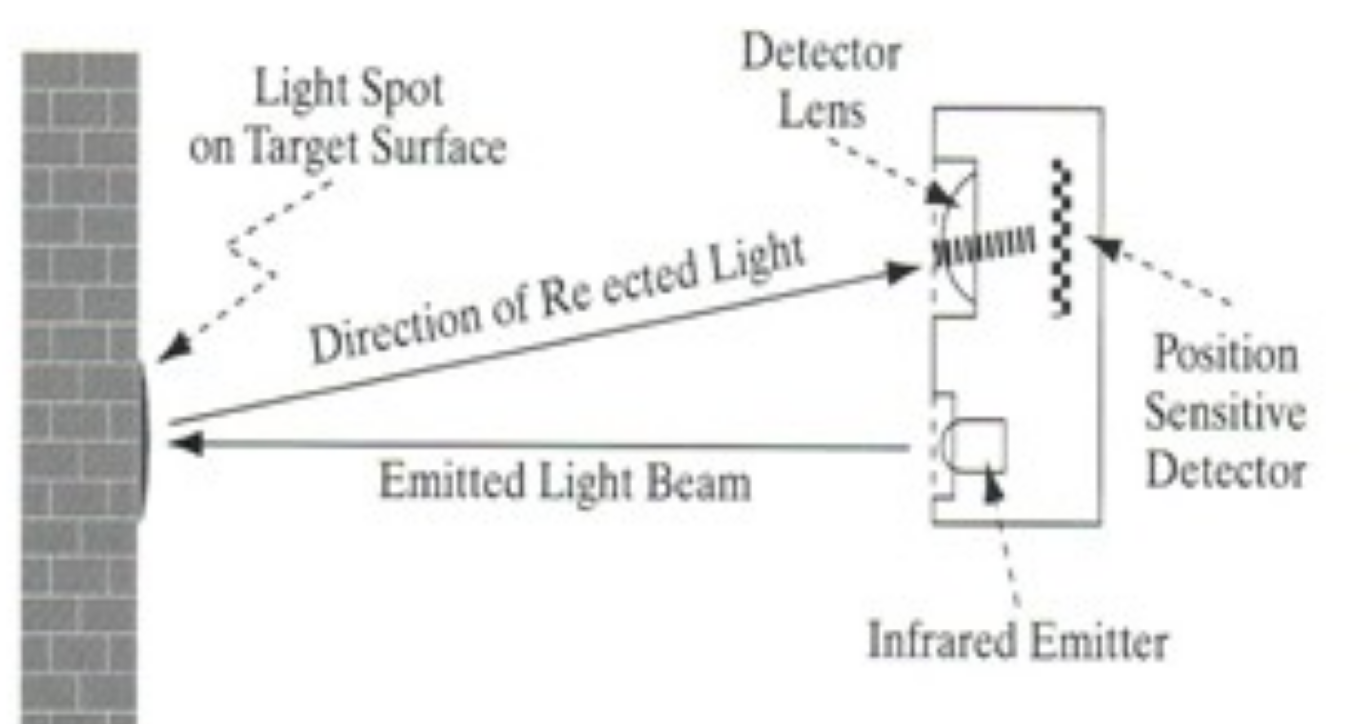
\includegraphics[width=2.5in]{ir}
			\caption{Infrared obstacle detection diagram}
			\label{fig:ir}
		\end{figure}
		Since the light beam needs to be reflected by an object, its reflectance is an important factor to take into account, since poor reflective objects could not be detected on time.  Also, some other natural or artificial sources of radiation such as the Sun may cause interferences. To improve the circuit's response to interferences the signal must be properly conditioned and modulated \cite{mod_control_bresciani, remotecontrol}.
		
		\subsection{Ultrasonic sensors}
		This devices, together with the IR sensors, allow measuring the distance from the vehicle to an obstacle. An ultrasonic sensor consists of a high-frequency sound emitter and a receiver. Both are electrical signals \textendash \ sound wave transducers, and their operation is similar to the IR sensors: the emitted wave is reflected by the obstacle, and when received, the distance to the obstacle can be calculated based on the time of flight (TOF) of the signal in the air, as can be seen in \figurename \ref{fig:ultrasonic}. Since the velocity of the sound in the air is known, just by knowing the time that passed between emission and reception, the distance to the obstacle can be known, according to (\ref{eq:ultrasonic_formula}). 
		
		\begin{equation} \label{eq:ultrasonic_formula}
		d\subb{obstacle} = \text{v}\subb{sound, air} \ \frac{TOF}{2}
		\end{equation}
		\begin{figure}
			\centering
			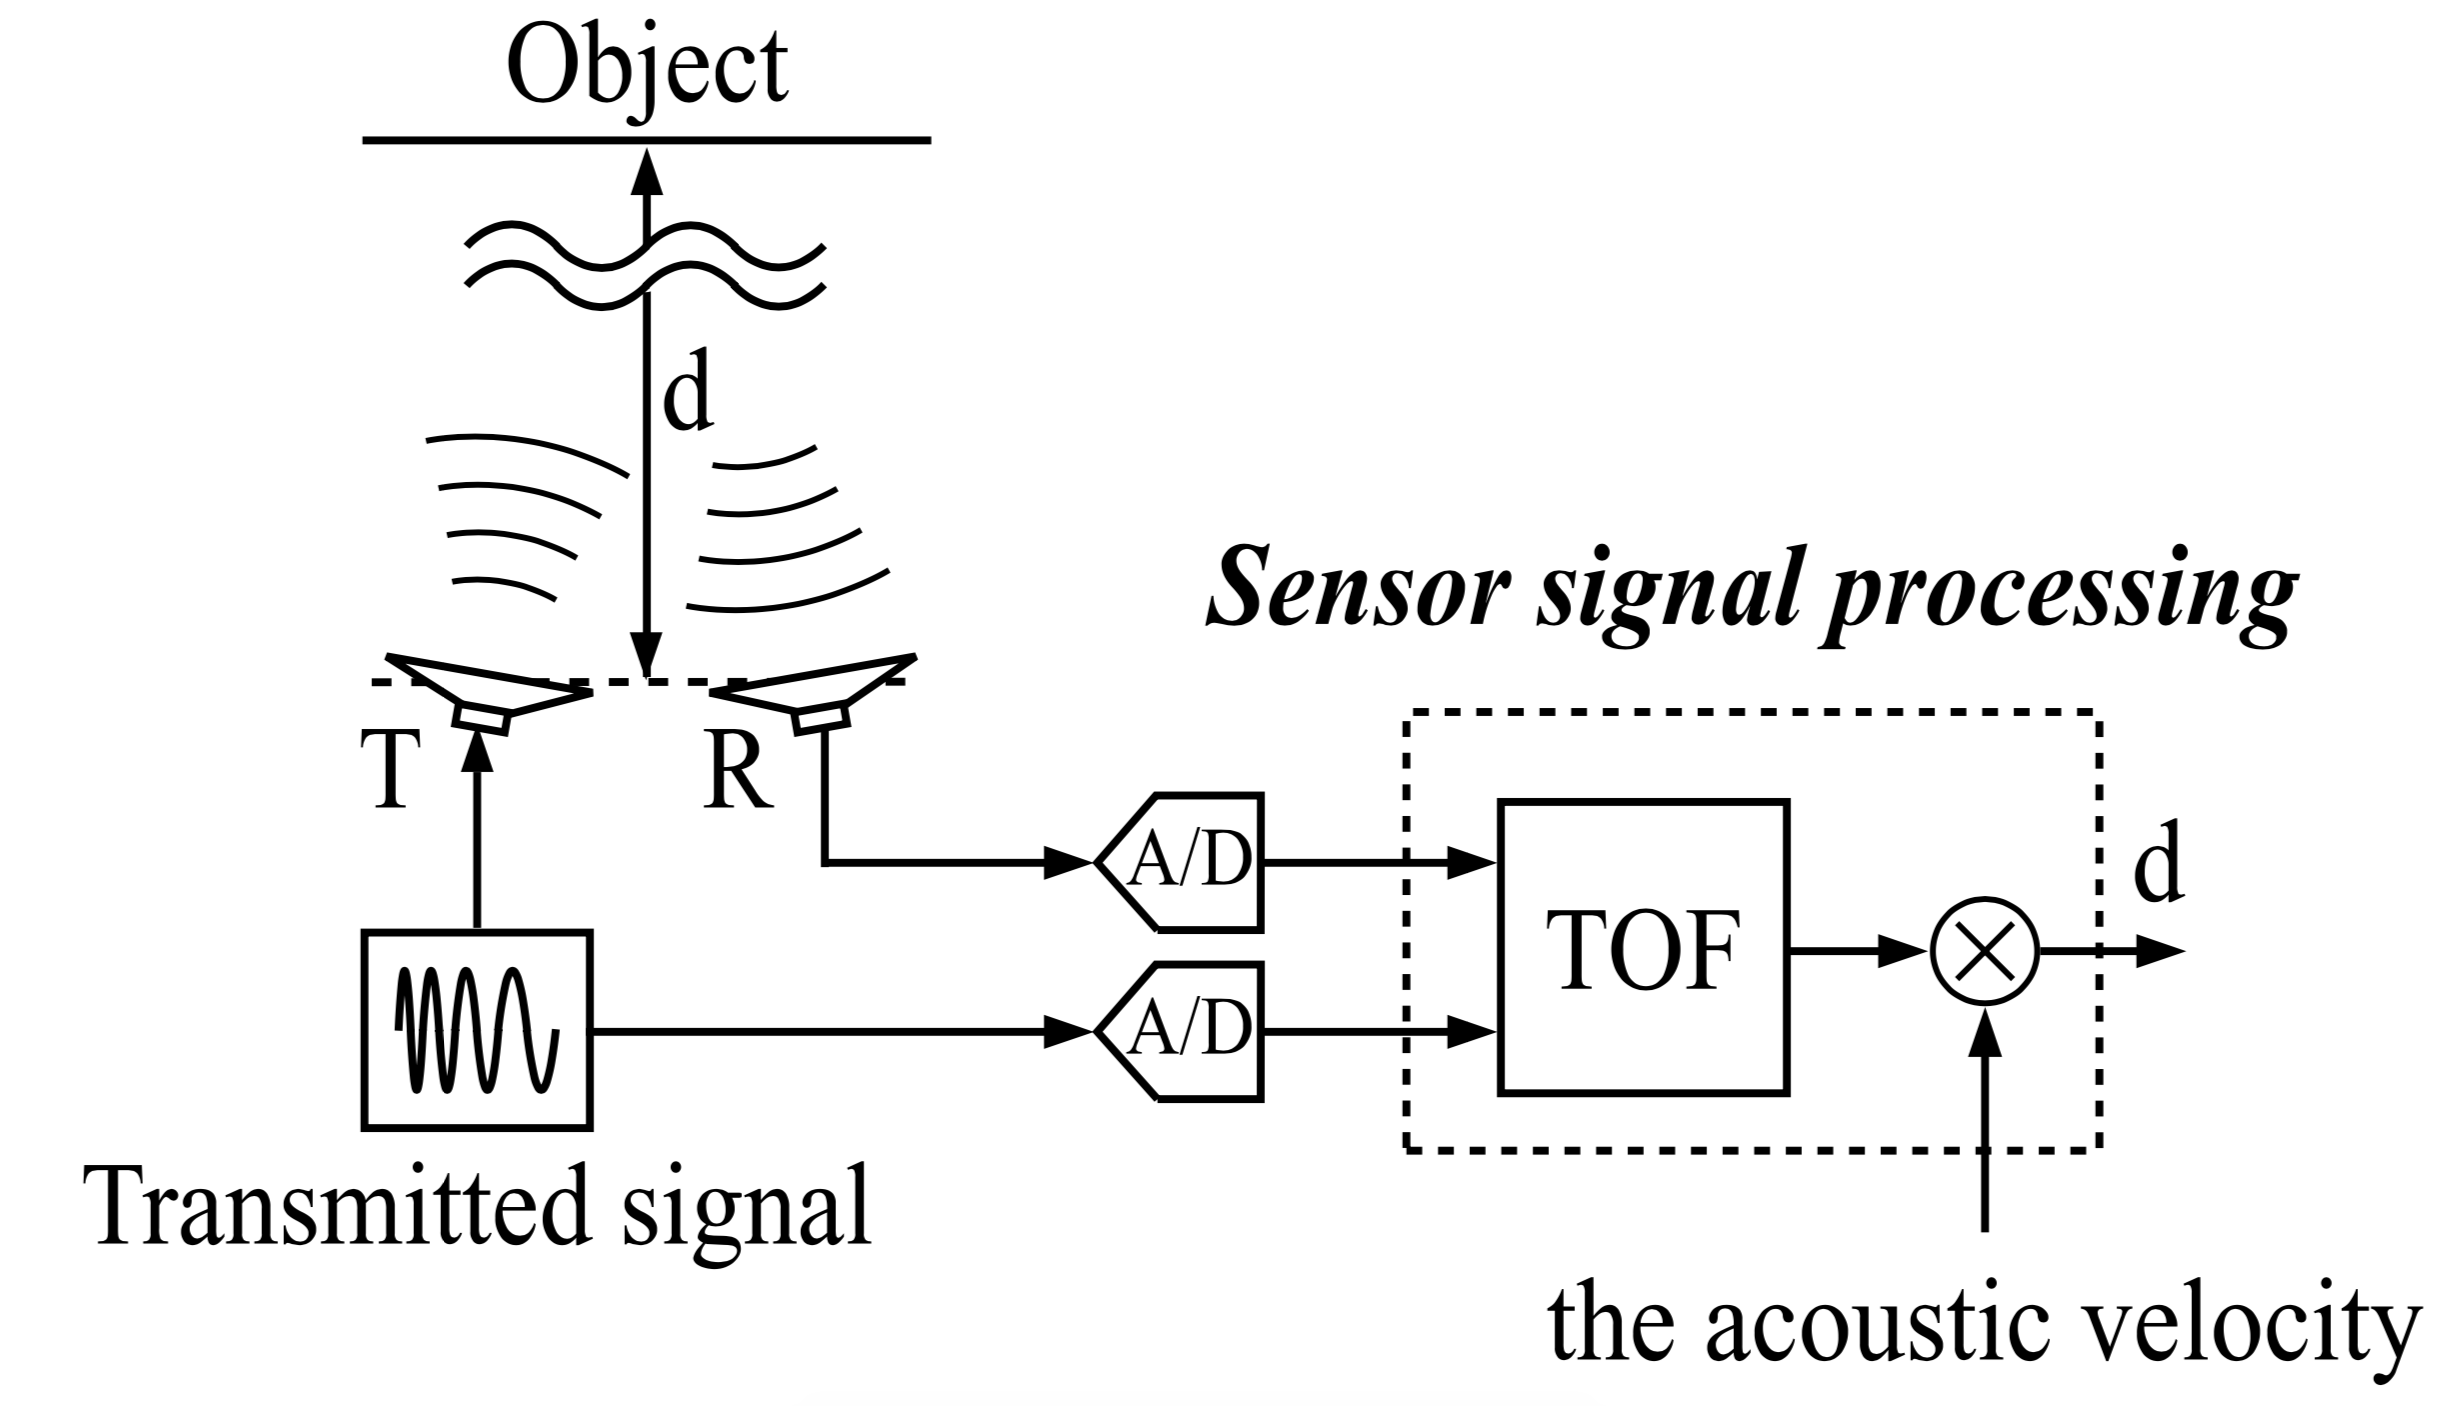
\includegraphics[width=2.5in]{ultrasonic2}
			\caption{Ultrasonic obstacle detection diagram, obtained from \cite{hirata2008cross}}
			\label{fig:ultrasonic}
		\end{figure}
		
		This sensors may also be used to measure the height of the UAV, that can be combined with a barometer to know both the relative and absolute altitude. According to Adarsh in \cite{AdarshS2016PcoI}, both IR and ultrasonic sensors have usually high correlation between the measured values, except for some specific materials. Both types have proven to be accurate when performing further processing techniques of the acquired data.
		
	\section{Quadcopter navigation}
	There are several methods to find the optimal path to follow from initial position to goal. In the case that is being studied in this paper, there are several UAVs flying towards their goals, in an environment filled with obstacles \cite{potfieldsmethod}.
	
	\begin{equation} \label{eq:pot_}
	cucu
	\end{equation}
	
	\section{Simulation}
	
	
	\section{Results}
	It's bloody impossible to do this.
	
	\section{Discussion, conclusion and Future development}
	
	
	
	% if have a single appendix:
	%\appendix[Proof of the Zonklar Equations]
	% or
	%\appendix  % for no appendix heading
	% do not use \section anymore after \appendix, only \section*
	% is possibly needed
	
	% use appendices with more than one appendix
	% then use \section to start each appendix
	% you must declare a \section before using any
	% \subsection or using \label (\appendices by itself
	% starts a section numbered zero.)
	%
	
	
	\appendices
	\section{Dynamics or something that's heavy on the maths goes here}
	Appendix one text goes here.
	
	% you can choose not to have a title for an appendix
	% if you want by leaving the argument blank
	\section{Something else but similar here, matlab code?}
	Appendix two text goes here.
	
	
	% use section* for acknowledgement
	\section*{Acknowledgment}
	
	Praising of Christos goes here!
	The authors would like to thank...
	TEST
	
	
	% Can use something like this to put references on a page
	% by themselves when using endfloat and the captionsoff option.
	\ifCLASSOPTIONcaptionsoff
	\newpage
	\fi
	
	
	
	% trigger a \newpage just before the given reference
	% number - used to balance the columns on the last page
	% adjust value as needed - may need to be readjusted if
	% the document is modified later
	%\IEEEtriggeratref{8}
	% The "triggered" command can be changed if desired:
	%\IEEEtriggercmd{\enlargethispage{-5in}}
	
	% references section
	
	% can use a bibliography generated by BibTeX as a .bbl file
	% BibTeX documentation can be easily obtained at:
	% http://www.ctan.org/tex-archive/biblio/bibtex/contrib/doc/
	% The IEEEtran BibTeX style support page is at:
	% http://www.michaelshell.org/tex/ieeetran/bibtex/
	\bibliographystyle{IEEEtran}
	% argument is your BibTeX string definitions and bibliography database(s)
	%\bibliography{Report}
	\bibliography{bib}
	
	
	
	% You can push biographies down or up by placing
	% a \vfill before or after them. The appropriate
	% use of \vfill depends on what kind of text is
	% on the last page and whether or not the columns
	% are being equalized.
	
	%\vfill
	
	% Can be used to pull up biographies so that the bottom of the last one
	% is flush with the other column.
	%\enlargethispage{-5in}
	
	
	
	% that's all folks
\end{document}


